\documentclass[10pt,twocolumn,hidelinks]{witseiepaper}

\usepackage{KJN}
\usepackage{algorithm2e}
\usepackage{graphicx}
\usepackage{caption}
\usepackage{subcaption}
\usepackage{hyperref}


\graphicspath{ {../../src/experiment}, {img}, {../../src/yagi-uda}}

\thispagestyle{plain}\pagestyle{plain}

\begin{document}

\title{Design, Prototyping, and Evaluation of a Directional Wi-Fi Antenna
    Using Simulation Models and Low-Cost Empirical Performance-Testing
    Techniques}

\author{Shivun Chinniah, Student Number: 2090476 \thanks{School of
        Electrical \& Information Engineering, University of the
        Witwatersrand, Private Bag 3, 2050, Johannesburg, South Africa} }

\abstract{This report documents the design, prototyping, and testing of a
    directional Wi-Fi antenna, as a part of the ELEN4001 High Frequency
    Techniques course at the University of the Witwatersrand. The design
    principles carried out were based on the methods described in
    \textit{Antennas in Practice} by Clark and Fourie
    \cite{clark_fourie_2002}. The antenna was designed using, tested,
    parameterized, theoretical models and thereafter was refined via the
    MATLAB (Antenna Toolbox) \cite{matlabantenna} simulation  software.
    Lastly the Prototype antenna was physically constructed and tested
    yielding promising results.}

\keywords{Antenna, Low-Cost, Wi-Fi, Yagi-Uda, MATLAB, RSSI}

\maketitle




\section{Introduction}

Wi-Fi routers are often designed to utilise 'omni-directional' antennas
which \textit{attempt} to radiate power isotropically  within a building
\cite{wifiantenna}. However this can be considered inefficient in cases
such as in long buildings where a router can only be placed at an extreme
end of the building. One solution to this problem is to increase the
overall transmitted Wi-Fi power within the building, by either increasing
the transmit power of the router, or by adding an additional router, making
this solution cost ineffective. Considering that the inefficiency arises as
power is radiated to areas where it is not needed (outside the building),
instead of areas where it would be deemed useful, a more cost effective
solution is to ensure that power is better 'directed'. Hence in this report
a directional antenna is designed with the intent of increasing the
range-of-use of a Wi-Fi Router within a building, under the constraint that
it is affordable for home users. Additionally this report will focus only
on the '2.4 GHz' Wi-Fi band, even though there also exists a '5 GHz' band
\cite{802.11}. It is assumed that by increasing the directivity of the
transmitting antenna that an improvement in signal quality will be
observed, despite despite the presence of obstacles. One could hypothesise
that if power is better directed to an area initially receiving relatively
low power, then the net power should increase as long the obstacles remain
the same.

This report will first discuss the design process of the antenna by
outlining its specifications to which antenna design theory can be applied
to derive a base-line antenna model. Thereafter the base-line model is
simulated, evaluated and then refined to ensure that the specifications are
met. A physical prototype is subsequently constructed, and tested by
gathering empirical measurements using inexpensive test equipment such as
smart phones and consumer Wi-Fi routers. Lastly the results from the
performance testing are evaluated to determine if the success criteria is
met. The success criteria being that: the antenna is directional, matched
correctly to the generator-transmission-line circuit (Wi-Fi router), and
that it is efficient enough to outperform the stock omni-directional
antenna regarding range-of-use.


\section{Antenna Design}

The design process of the antenna begins with defining: its operational
specifications, and its type by considering potential construction material
and Wi-Fi hardware; physical dimensions are then calculated based on the
selected antenna type. Lastly a matching circuit is designed to ensure that
the antenna operates efficiently.

\subsection{Specifications}
Wi-Fi Routers follow the IEEE 802.11 \cite{802.11} Standard, which dictates
antenna and connection media specifications, RF Frequency bands, and
channel allocations on these bands (table \ref{tab:channel}). The specific
band at which the antenna should operate is between $2.4$ and $2.4835$ GHz
in most countries; however in other countries such as Japan it should
operate between $2.471$ and $2.497$ GHz. Hence the designed antenna should
have a bandwidth of 500 MHz and and should be centred at 2.45 GHz. The
expected impedance at the connection terminals of the Wi-Fi router is
$50\ohm$.
\begin{table}[!h]
    \begin{center}
        \caption{2.4 GHz Wi-Fi Channel Allocations centred at Frequency $f$}
        \label{tab:channel}
        \resizebox{0.48\textwidth}{!}{\begin{tabular}{| l | c c c c c c }
                \hline
                Channel No. & 1    & 2    & 3    & 4    & 5    & 6 ...
                \\
                $f$ (MHz)   & 2412 & 2417 & 2422 & 2427 & 2432 & 2437 ...
                \\
                \hline
            \end{tabular}}
    \end{center}
    \begin{center}
        \resizebox{0.48\textwidth}{!}{ \begin{tabular}{ c c c c c c c c | }
                \hline
                ...  7    & 8    & 9    & 10   & 11   & 12   & 13   & 14
                \\
                ...  2442 & 2447 & 2452 & 2457 & 2462 & 2467 & 2472 & 2484
                \\
                \hline
            \end{tabular}}
    \end{center}
\end{table}
It is important to note that indoor Wi-Fi antennas typically have a gain of
between 0 to 6 dBi \cite{wifiantenna}. Gain is defined as the the product
of \textit{efficiency} and \textit{directivity}. To recall:
\textit{efficiency} is the ratio of the power inputted to the power
outputted of a system; \textit{directivity} the measure of how much an
antenna is able to 'focus' the power from one angular region to another.
\textit{Directivity} is presented as a logarithmic ratio relative to the
directivity of an isotropic source (a source radiates perfectly in all
directions) using the units 'dBi' \cite[p. 18-20]{clark_fourie_2002}.

Based on the above and the previously described project constraints the
following specifications were derived and are listed in table
\ref{tab:specs}.

\begin{table}[!h]
    \begin{center}
        \caption{Specifications of Designed Antenna}
        \label{tab:specs}
        \begin{tabular}{ l c }
            \hline
            \multicolumn{1}{c}{Specification} &
            \multicolumn{1}{c}{Description}                 \\
            \hline
            Frequency Range (MHz)             & 2400 - 2500 \\

            Design Frequency (MHz)            & 2450        \\

            Maximum VSWR                      & 2:1         \\

            Input Impedance ($\ohm$)          & 50          \\

            Cost (ZAR)                        & <100        \\

            Gain (dBi)                        & >6          \\

            \hline
        \end{tabular}

    \end{center}

\end{table}

The cost price of the antenna assumes that scavenged parts cost 0 ZAR
(South African Rand), and that coaxial cable and corresponding connectors
need to be purchased with a budget of 100 ZAR; also assumed to be
"affordable for home users."

\subsection{Theory: Yagi-Uda Antenna}
\label{theory}
The type of antenna chosen is the directional Yagi-Uda as it is simple to
construct with material that is readily found within a house hold. It
consists of an single \textit{excited element} from which the antenna is
fed, a \textit{reflector} element, and a number of \textit{director}
elements. As literature \cite[p. 67-68]{clark_fourie_2002} explains the
boom (total) length is proportional to the resulting directivity, however
is inversely proportional the resulting operational bandwidth. Figure
\ref{yagi4} shows a the core elements and length parameters of a 4-director
Yagi-Uda antenna, from which an $N$-element antenna follows closely.

\begin{figure}
    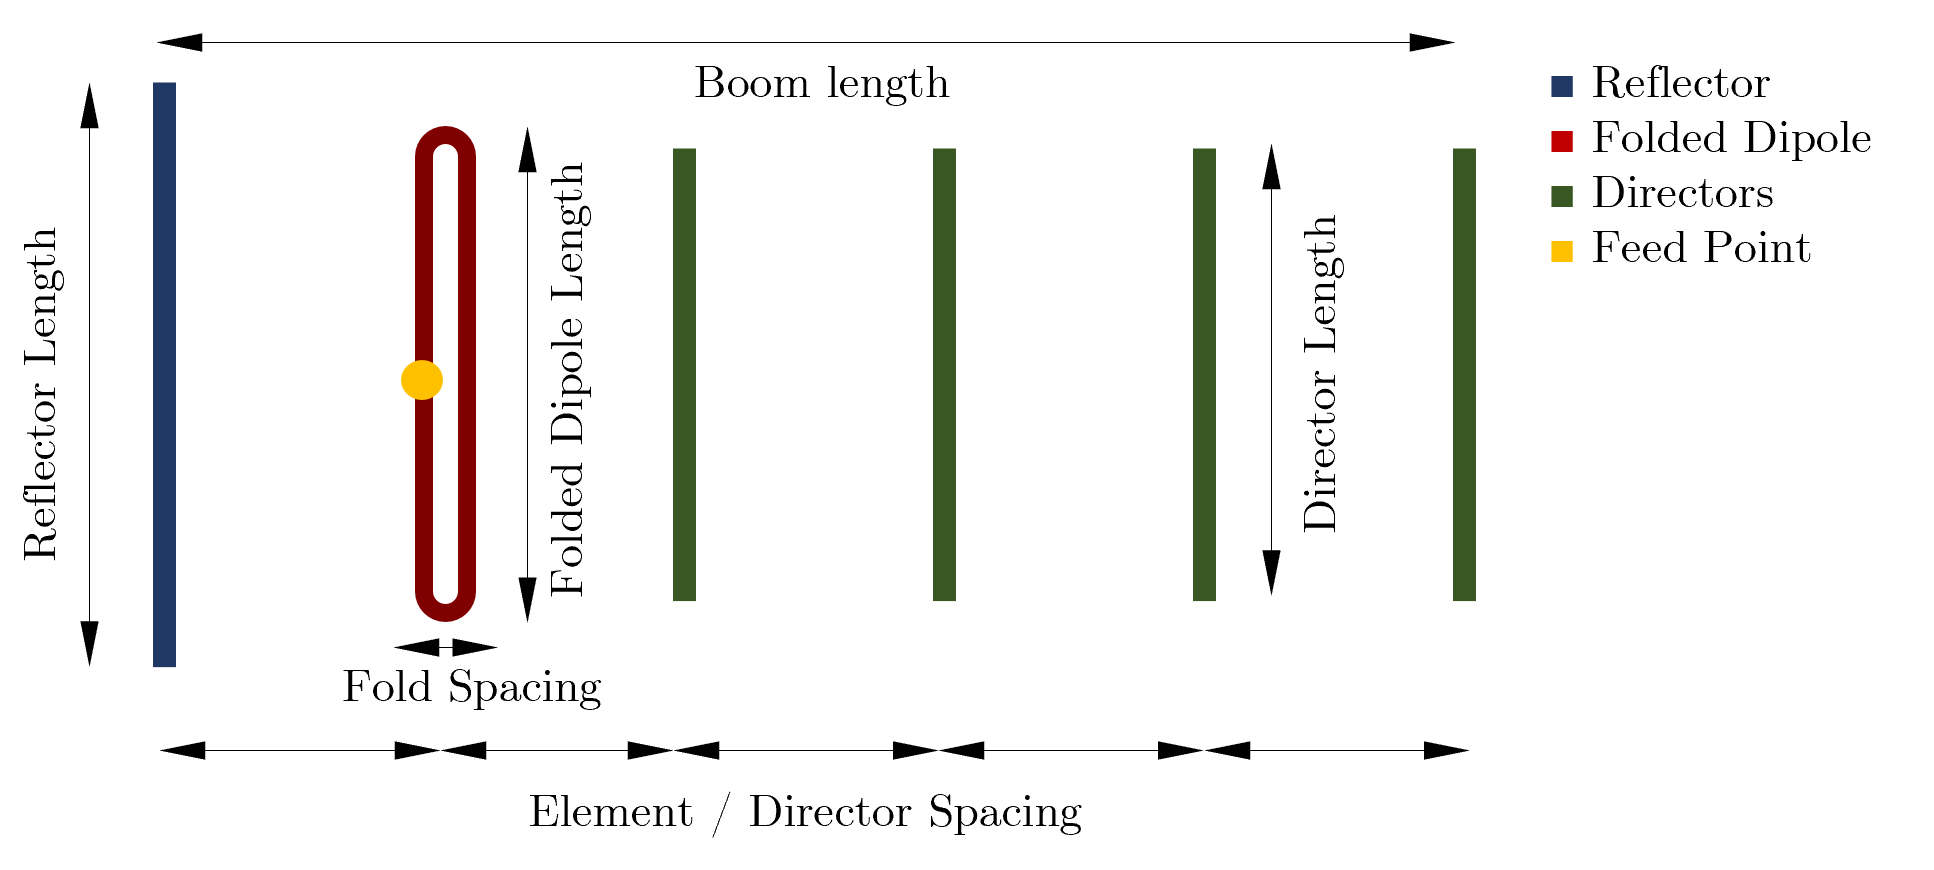
\includegraphics[width=\linewidth]{yagiuda4.png}
    \caption{Diagram of the Parameterized Elements of a 4-director Yagi-Uda Antenna}
    \label{yagi4}
\end{figure}

The design approach specified in \cite[p. 69]{clark_fourie_2002} mentions
two sources: the NBS technical report published in 1976 \cite{NBS}, and the
\textit{Yagi-antenna Design} \cite{lawson} text published ten years later.
It is noted that the NBS report had computed optimal, varying, lengths for
the director elements, however it was shown that using the average length
of the directors also performed well \cite{lawson}, furthermore simplifying
the antenna fabrication process as the director lengths are all the same.

Some of these elements lengths, specifically for: a 4-director,
10-director, and a 15-director Yagi-Uda configuration are presented in
table \ref{tab:yagielem} in units of wavelength ($\lambda$) and mm. It is
important to note that element lengths presented in table
\ref{tab:yagielem} are designed for an element diameter of 0.008$\lambda$
which equates to approximately 0.98mm, hence a correction factor is
required if a different diameter is used. These configurations are are
considered as they offer a range of design options from which either
bandwidth or directivity can be maximised, with the 10-director
configuration serving as a relatively neutral starting point.

The excited element commonly takes the form of a Folded Dipole antenna,
however the overall length of this antenna differs from the case where
there are no directors or reflectors \cite[p. 69]{clark_fourie_2002}. The
recommended spacing between the the folded portion of the antenna is less
than a twentieth of its length \cite[p. 506]{balanis2005antenna}.

\begin{table}[!h]
    \begin{center}
        \caption{Recommended lengths for the elements of a 4-director,
            10-director, and 15-director Yagi-Uda Antenna at 2.45 GHz
            \cite[p. 69]{clark_fourie_2002}}
        \label{tab:yagielem}
        \resizebox{0.48\textwidth}{!}{\begin{tabular}{|l|cc|cc|cl|}
                \hline
                Element                          &
                \multicolumn{2}{c|}{4-director}  &
                \multicolumn{2}{c|}{10-director} &
                \multicolumn{2}{c|}{15-director}
                \\ \hline
                                                 &
                \multicolumn{1}{c|}{($\lambda$)} & (mm)  &
                \multicolumn{1}{c|}{($\lambda$)} & (mm)  &
                \multicolumn{1}{c|}{($\lambda$)} &
                \multicolumn{1}{c|}{(mm)}
                \\ \hline
                Reflector                        &
                \multicolumn{1}{c|}{0.482}       & 59.02 &
                \multicolumn{1}{c|}{0.482}       & 59.02 &
                \multicolumn{1}{c|}{0.482}       & 59.02   \\
                Spacing                          &
                \multicolumn{1}{c|}{0.200}       & 24.49 &
                \multicolumn{1}{c|}{0.200}       & 24.50 &
                \multicolumn{1}{c|}{0.200}       & 24.50   \\
                Director                         &
                \multicolumn{1}{c|}{0.427}       & 51.29 &
                \multicolumn{1}{c|}{0.402}       & 49.22 &
                \multicolumn{1}{c|}{0.395}       & 48.37   \\
                Exciter                          &
                \multicolumn{1}{c|}{0.378}       & 46.29 &
                \multicolumn{1}{c|}{0.382}       & 46.72 &
                \multicolumn{1}{c|}{0.396}       & 48.49   \\ \hline
                R/D                              &
                \multicolumn{2}{c|}{1.289}       &
                \multicolumn{2}{c|}{1.199}       &
                \multicolumn{2}{c|}{1.22}
                \\ \hline
                Suited for                       &
                \multicolumn{2}{c|}{Bandwidth}   &
                \multicolumn{2}{c|}{Neutral}     &
                \multicolumn{2}{c|}{Gain}
                \\ \hline
            \end{tabular}}
    \end{center}

\end{table}

\subsection {Matching Circuit}
A matching circuit is often required to ensure that the antenna has the
same impedance of the rest of the high frequency circuit. This is important
because if an antenna is not properly matched to its driving circuit then
power is reflected back to the driving electronics potentially causing
damage. This would also mean that the antenna is less efficient as only a
portion of the power is inputted to the antenna to be radiated, thus the
antenna will also have a lower gain. Two methods are considered to match
the antenna to the 50$\ohm$ Wi-Fi router port: a half-wave balun, and a
stub matching circuit as posed in \cite[p. 33,36]{clark_fourie_2002}.

It is expected that the impedance of a Folded Dipole-driven Yagi-Uda
antenna is on the order of 200$\ohm$, hence a 4:1 impedance transformer
should match the antenna to a 50$\ohm$ line. Using a half-wave balun this
is precisely what is achieved \cite[p. 69]{clark_fourie_2002}.

In the event that the resulting antenna's impedance is not near 200$\ohm$,
the a stub matching circuit would have to be considered. Using such a
circuit allows for a variable impedance transformation to occur, albeit for
a narrow bandwidth. One favours the half wave balun as it is more simple to
implement physically, as it only requires cutting a piece of coaxial cable
to length, where as the stub matching circuit would require multiple
calculations, measurements, cuts and joins.

\section{Simulation and Refinement}
\label{simref}

The recommended element lengths discussed in section \ref{theory} were
inputted into a parametrised model of a Folded Dipole-driven Yagi-Uda
antenna for the 10-director case using MATLAB's Antenna Toolbox
\cite{matlabantenna}. Initial simulations showed that a maximum directivity
of 11 dBi with a bandwidth of nearly 1 GHz (assuming matched conditions)
was achievable. However the center frequency was not 2.45 GHz. According to
\cite[p. 69]{clark_fourie_2002} the exciter element's length -- the folded
dipole -- dictates resonance, hence it was tuned to ensure matching (zero
reactance) at the center frequency using a binary search-based optimisation
algorithm.

It was decided that the number of directors, and thus the boom length
should be increased to 15 to make a trade-off between the larger than
necessary bandwidth for a larger gain instead. Similar to the 10-director
case, using the theoretical lengths yielded expected results, however the
folded dipole length had to be tuned to meet the required center frequency.

The final dimensions for the refined antenna are the same as those listed
in table \ref{tab:yagielem} for the 15-element case as a 1mm element
diameter was used (no correction factor). However the folded dipole
dimension are as follows: the length is 53.1mm with a fold spacing of 1mm.

\begin{figure}
    \includegraphics[width=0.85\linewidth]{impedance.eps}
    \caption{Antenna Input Impedance}
    \label{impedance}
    \vspace{-0.3cm}
\end{figure}

Figure \ref{impedance} shows the input impedance for the refined antenna,
it can be seen that the impedance is in the order of 200$\ohm$ for the 2450
to 2500 MHz range, hence a halve wave balun may be used. It can also be
seen that the antenna is designed to have zero reactance at the center
frequency.
\begin{figure}
    \includegraphics[width=0.85\linewidth]{vswr.eps}
    \vspace{-0.1cm}
    \caption{Impedance Bandwidth Relative to 50$\ohm$ and 200$\ohm$}
    \label{vswr}
    \vspace{-0.35cm}
\end{figure}

The impedance bandwidth was determined using figure \ref{vswr}. The
obtained bandwidth of antenna is under 300 MHz (~2.3 to 2.6 GHz) assuming
matched conditions (200$\ohm$ figure \ref{vswr}), whereas the antenna does
not meet the 2:1 VSWR requirement if it were to be connected to a Wi-Fi
router without a matching circuit (50$\ohm$ figure \ref{vswr}).
\begin{figure}
    \includegraphics[width=0.85\linewidth]{gain2.eps}
    \caption{Gain Bandwidth at 90$\degree$ Azimuth (dBi)}
    \label{gainbw}
    \vspace{-0.35cm}
\end{figure}

Figure \ref{gainbw} shows that there is a large gain bandwidth that meets
the 6 dBi specification, but more importantly that the Gain of the antenna
is maximised and consistent at the required frequency band. This figure was
generated by performing a frequency sweep at maximum gain coordinate, which
was obtained by the radiation pattern presented in figure \ref{antpatt}.
Figure \ref{antpatt} shows that a the antenna is indeed directional, and
that maximum gain of 14.16 dBi is observed along the boom axis at away from
last director element.

\begin{figure*}
    \centering
    \begin{subfigure}{0.3\linewidth}
        \includegraphics[width=\textwidth]{azimuth.eps}
        \vspace{-.2cm}
        \subcaption{Azimuth Pattern (dBi)}
    \end{subfigure}
    \begin{subfigure}{0.3\linewidth}
        \includegraphics[width=\textwidth]{elevation.eps}
        \vspace{-.5cm}
        \subcaption{Elevation Pattern (dBi)}
    \end{subfigure}
    \begin{subfigure}{0.3\linewidth}
        \includegraphics[width=\textwidth]{3dplot.eps}

        \subcaption{3D Radiation Pattern}
    \end{subfigure}
    \caption{Antenna Radiation Pattern}
    \label{antpatt}
\end{figure*}

\section{Prototyping}
Based on the derived theoretical antenna model, and simulation results a
physical antenna was constructed and then tested to verify that the
intended design specifications were met.

\subsection{Construction}
A prototype antenna was constructed using 1mm steel rods, extracted from an
old electric fly-swatter. fifteen director elements and a reflector element
were cut to the values presented in table \ref{tab:yagielem} (15-element).
A metal file and calipers were used to shave the elements to 0.5mm
accuracy. The rod for the folded dipole was cut and then folded to the
length determined in the \hyperref[simref]{\textit{Simulation and
Refinement}} section. This was done to 0.8 mm accuracy, with the spacing
between the fold being 0.2mm accurate. The finished elements are shown in
Appendix, figure \ref{fig:cutelem}.

To connect the designed antenna to a Wi-Fi router, RG 174 A/U coaxial
cable\cite{rg174}, and compatible Reverse-Polarity SMA connectors were
procured for, a total cost of 45 ZAR.

To make the half wave balun transformer a piece of coaxial cable was cut to
length, taking the velocity factor into account. Equation \ref{equ:balun}
was used to determine the length in mm. The using a velocity factor of 0.66
\cite{rg174}, the resulting length of coaxial cable is 40.4mm. A slightly
longer piece of coaxial cable was cut so that the braid, and inner
conductor could be exposed for soldering, however the length of the
remaining sheath matched the calculated length. The balun is shown in
Appendix, figure \ref{fig:coaxbalun}.
\vspace{-0.1cm}
\begin{equation}
    \label{equ:balun}
    l_{mm}=\frac{300 \times VF}{2f_{MHz} } \times 10^3
    \vspace{-0.25cm}
\end{equation}

The next step of construction was to mount the elements to a plastic 3D
printed boom which spaced the elements according to
table\ref{tab:yagielem}. And lastly the coaxial cable with crimped RP-SMA
connector and balun was soldered to the feed point of the folded dipole
(Appendix, figure \ref{fig:feedpoint}). The constructed prototype is shown
in figure \ref{fig:prototype}.

\begin{figure}
    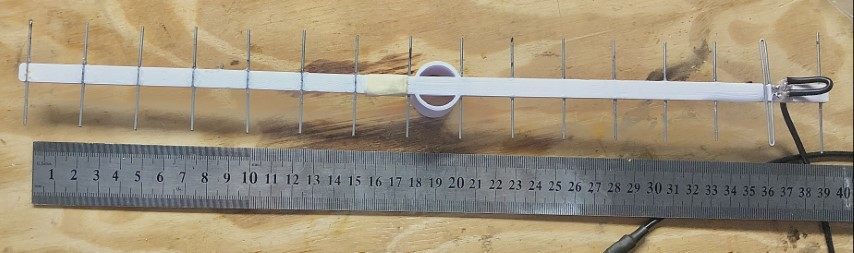
\includegraphics[width=.99\linewidth]{antenna.jpg}
    \caption{Constructed Prototype Antenna}
    \label{fig:prototype}
    \vspace{-0.35cm}
\end{figure}

\subsection{Testing}
To test the designed antenna a Wi-Fi router with external
antenna-connection ports is used. The model of the Wi-Fi Router is a
\textit{Tenda 3G226R+}, which supports the IEEE 802.11 standard and has two
3 dBi antennas\cite{tenda}. One stock antenna is used as a reference to
determine the the directivity of the designed antenna.

\subsubsection{Experimental Proceedure}~\\
\label{expproc}
The experiment involves gathering data points that would allow for a
pseudo-azimuth plot to be created for both antennas. The radiated power
received from a smartphone -- positioned at various angles and at fixed
distance away from the antennas -- is reported via its hardware's Received
Signal Strength Indicator (RSSI). An Android application called
\textit{WiFi Analyzer} \cite{wifianalyzer} is used to obtain an RSSI. The
RSSI is expressed in dBm (power received relative to a milliwatt). Hence by
gathering enough data points around the router a maximum signal intensity,
and an approximation of the falfield radiation pattern can be determined.

One can conclude that the maximum RSSI obtained (dBm) for the stock antenna
is proportional to its directivity (dBi); meaning the difference of the
maximum RSSI values measured for the stock and the designed antennas should
also be the difference of their Gains.

\begin{figure}
    \centering
    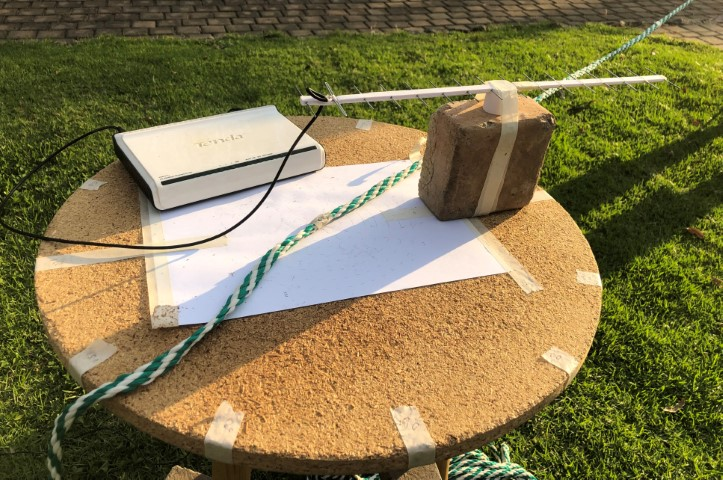
\includegraphics[width=0.4\textwidth]{experimental setup.jpg}
    \caption{Experimental Setup -- Prototype Antenna on
        30$\degree$-interval marked table, with 5m Rope and Wi-Fi Router}
    \label{fig:designexp}
    \vspace{-0.1cm}
\end{figure}


\subsubsection{Results}~\\
The described experimental procedure was conducted by taking 12
measurements separated $30\degree$ apart at a constant radius of 5m. Figure
\ref{fig:designexp} shows the prototype antenna on the marked experiment
table which has a 5m length of rope nailed down to the centre. The
transmitter power of the Wi-Fi Router was limited to 25 percent, and the
router was configured to broadcast on Channel 6. The radius and transmitter
power were set so as to ensure that all measurements would lie within the
-20 dBm and -100 dBm scale of the hardware-reported RSSI. Figure
\ref{empirical} presents the empirical results that were gathered for the
designed and stock antennas. It is important to note that the measured
values often fluctuated by 3 dBm, and a measurement was only recorded once,
the RSSI value settled for at least 5 seconds.

The maximum RSSI obtained for the stock antenna was -48 dBm at
240$\degree$, and -34 dBm at 90$\degree$ for the designed antenna.

\begin{figure}
    \centering
    \includegraphics[width=0.99\linewidth]{measure_dBm_5m_25pow.eps}
    \vspace{-1cm}
    \caption{Measured RSSI (dBm) as observed from various angles for Stock
        and Designed Antennas at a distance of 5m with 25\% transmit power
        (Channel 6)}
    \label{empirical}
    \vspace{-0.5cm}
\end{figure}


\section{Discussion}
As is seen in figure \ref{empirical} the prototype antenna does appear to
be significantly more directional than the stock antenna. This figure also
hints that the efficiency of the designed antenna is of the same order of
magnitude as the stock antenna since the stock antenna's maximum RSSI was
surpassed; hence it can be assumed that the prototype antenna is
sufficiently matched to the generator circuit. Assuming high efficiency
(\~90\%) an estimate of the prototype antenna's gain can be calculated as
17$\pm$2 dBi as described in \hyperref[expproc]{\textit{Experimental
Proceedure}}. This result does agree with the simulated result of 14.16 dBi
considering the limited precision of the test equipment used.

Thus it can be said that the success criteria of the project has been met,
however it must be noted that there has only been limited evidence that
supports that the prototype produces similar results to the simulations. A
significant limitation of the prototype is that thin coaxial cable was
used, which at 2.45 GHz frequencies imposes significant
attenuation\cite{rg174}.

There is much opportunity for future work, such as conducting the
experiment using different Wi-Fi Channels to determine if the antenna
operates efficiently for its full specified frequency range. Other work
includes investigating, and researching whether the Android measurement
application compensates for Automatic Gain Control, as this may explain the
great amount of fluctuation at certain testing angles. Lastly it has only
been assumed that the range of the Wi-Fi router is extended due to evidence
of increased gain and directivity, this calls for another experiment to be
conducted to measure this directly.
\section{Conclusion}
In this report a directional Yagi-Uda Wi-Fi antenna was successfully
designed using theory, and simulation models. An affordable prototype
antenna was then constructed, and tested using inexpensive test equipment.
The results from the testing experiment showed that the prototype antenna
had satisfied most design specifications, however future work must be
conducted to verify consistency in performance for the rest of its
specified frequency range.

\bibliographystyle{witseie}
{\small
    \bibliography{References}
}
\newpage
\onecolumn
\appendix
\pagestyle{empty}

% \section{Photographs}

\begin{figure}[hbt!]
    \centering
    \begin{subfigure}{0.40\linewidth}
        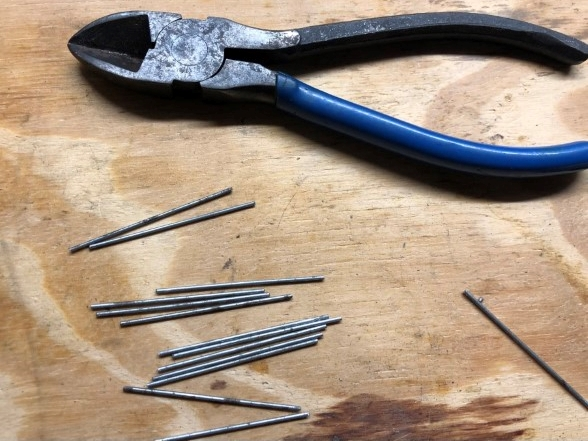
\includegraphics[width=\textwidth]{cutters.jpg}
        \subcaption{Steel Rod Cutting Tool}
    \end{subfigure}
    \begin{subfigure}{0.40\linewidth}
        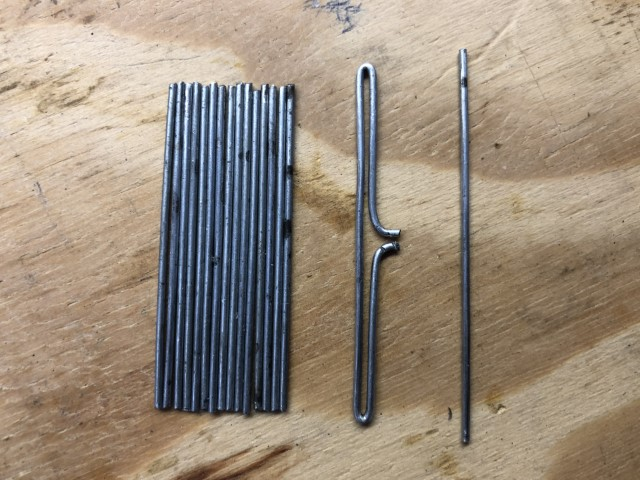
\includegraphics[width=\textwidth]{cut-elements.jpg}
        \subcaption{Cut and Folded Elements}
    \end{subfigure}
    \caption{Yagi-Uda Element Fabrication}
    \label{fig:cutelem}
\end{figure}
% \begin{figure*}[h!] \centering
%     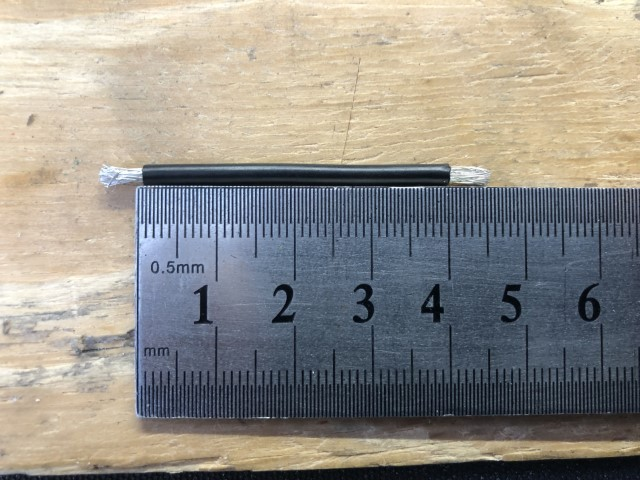
\includegraphics[width=0.4\textwidth]{balun.jpg} \caption{Coaxial
%     Cable to form Half-wave Balun (40.4mm)} \label{fig:coaxbalun}
%     \end{figure*}

\begin{figure}[h!]
    \begin{minipage}[c]{0.5\linewidth}
        \centering
        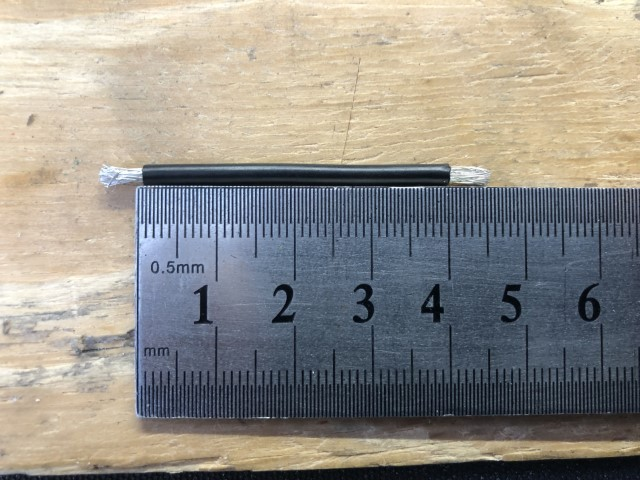
\includegraphics[width=0.9\linewidth]{balun.jpg}
        \caption{Coaxial Cable to form Half-wave Balun (40.4mm)}
        \label{fig:coaxbalun}
    \end{minipage}\hfill
    \begin{minipage}[c]{0.5\linewidth}
        \centering
        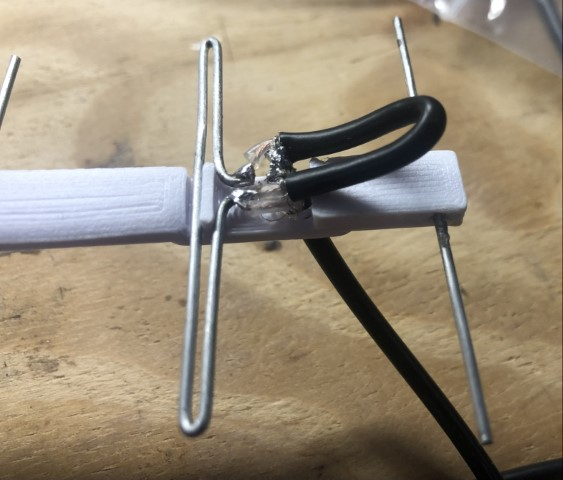
\includegraphics[width=0.9\linewidth]{feedpoint.jpg}
        \caption{Prototype Antenna Feed-Point}
        \label{fig:feedpoint}
    \end{minipage}

\end{figure}

\begin{figure*}[h!]
    \centering
    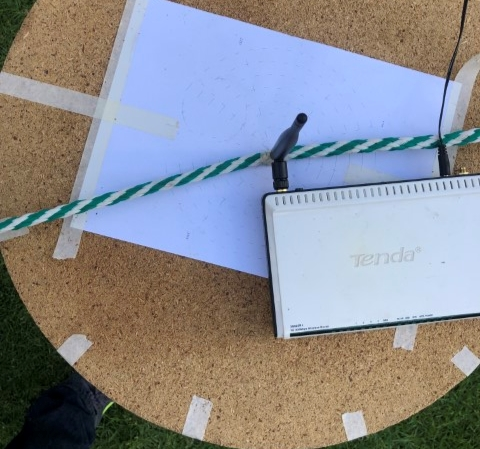
\includegraphics[width=0.5\textwidth]{stock-experiment.jpg}
    \caption{Experimental Setup for Stock Antenna}
    \label{fig:stockset}
\end{figure*}

\end{document}